\section{Question 1}
\begin{enumerate}[label=(\alph*)]
    \item Write down the definition of \textbf{norm} for a vector space.
        \begin{solution}{}{}
            Let $\mX$ be a real vector space. A nonnegative-valued function $\norm{\cdot}: \mX\to\RR$ is called a norm if $\forall\vx,\vy\in\mX, \lambda\in\RR$
            \begin{itemize}
                \item $\norm{\lambda\vx}=\abs{\lambda}\norm{\vx}$ (absolutely homogeneous);
                \item $\norm{\vx+\vy}\leq\norm{\vx}+\norm{\vy}$ (triangle inequality);
                \item $\norm{\vx}=0\Rightarrow\vx =\va{0}$ (positive definite).
            \end{itemize}
            Moreover, the vector norm $\norm{\cdot}_p$ for $p=1,2,\ldots$ is defined as
            \[
                \norm{\vx}_p = \qty(\sum_{1\leq i\leq n}\abs{x_i}^p)^{1/p}.
            \]
            And the pair $(\mX, \norm{\cdot})$ is called a normed space.
        \end{solution}
    \item Given $\vx\in\RR^n$, show that followings are norm on $\RR^n$.
        \begin{enumerate}[label=\roman*.]
            \item $\norm{\vx}_\infty=\max_{1\leq i\leq n}\abs{x_i}$;
                \begin{solution}{}{}
                    \begin{itemize}
                        \item $\norm{\lambda\vx}_\infty=\max_{1\leq i\leq n}\abs{\lambda x_i}=\abs{\lambda}\max_{1\leq i\leq n}\abs{x_i}=\abs{\lambda}\norm{\vx}_\infty$
                        \item $\norm{\vx+\vy}_\infty=\max_{1\leq i\leq n}\abs{x_i+y_i}\leq\max_{1\leq i\leq n}\abs{x_i}+\max_{1\leq i\leq n}\abs{y_i}=\norm{\vx}_\infty+\norm{\vy}_\infty$
                        \item $\norm{\vx}_\infty=\max_{1\leq i\leq n}\abs{x_i}=0\Rightarrow\abs{x_i}=0\text{ where $1\leq i\leq n$}\Rightarrow\vx =\va{0}$
                    \end{itemize}
                \end{solution}
            \item $\norm{\vx}_1=\sum_{1\leq i\leq n}\abs{x_i}$;
                \begin{solution}{}{}
                    \begin{itemize}
                        \item $\norm{\lambda\vx}_1=\sum_{1\leq i\leq n}\abs{\lambda x_i}=\abs{\lambda}\sum_{1\leq i\leq n}\abs{x_i}=\abs{\lambda}\norm{\vx}_1$
                        \item $\norm{\vx+\vy}_1=\sum_{1\leq i\leq n}\abs{x_i+y_i}\leq\sum_{1\leq i\leq n}\abs{x_i}+\sum_{1\leq i\leq n}\abs{y_i}=\norm{\vx}_1+\norm{\vy}_1$
                        \item $\norm{\vx}_1=\sum_{1\leq i\leq n}\abs{x_i}=0\Rightarrow\abs{x_i}=0\text{ where $1\leq i\leq n$}\Rightarrow\vx =\va{0}$
                    \end{itemize}
                \end{solution}
            \item $\norm{\vx}_2=\qty(\sum_{1\leq i\leq n}\abs{x_i}^2)^{1/2}$.
                \begin{solution}{}{}
                    \begin{itemize}
                        \item $\norm{\lambda\vx}_2=\qty(\sum_{1\leq i\leq n}\abs{\lambda x_i}^2)^{1/2}=\abs{\lambda}\qty(\sum_{1\leq i\leq n}\abs{x_i}^2)^{1/2}=\abs{\lambda}\norm{\vx}_2$
                        \item $\norm{\vx+\vy}_2=\qty(\sum_{1\leq i\leq n}\abs{x_i+y_i}^2)^{1/2}\leq\qty(\sum_{1\leq i\leq n}\abs{x_i}^2)^{1/2}+\qty(\sum_{1\leq i\leq n}\abs{y_i}^2)^{1/2} = \norm{\vx}_2+\norm{\vy}_2$
                        \item $\norm{\vx}_2=\qty(\sum_{1\leq i\leq n}\abs{x_i}^2)^{1/2}=0\Rightarrow\sum_{1\leq i\leq n}\abs{x_i}^2\Rightarrow\vx =\va{0}$
                    \end{itemize}
                \end{solution}
        \end{enumerate}
        Plot the regions for $\norm{\vx}_p\leq 1$ in $\RR^2$ for $p=\infty,1,2$ respectively.
        \begin{figure}[H]
            \centering
            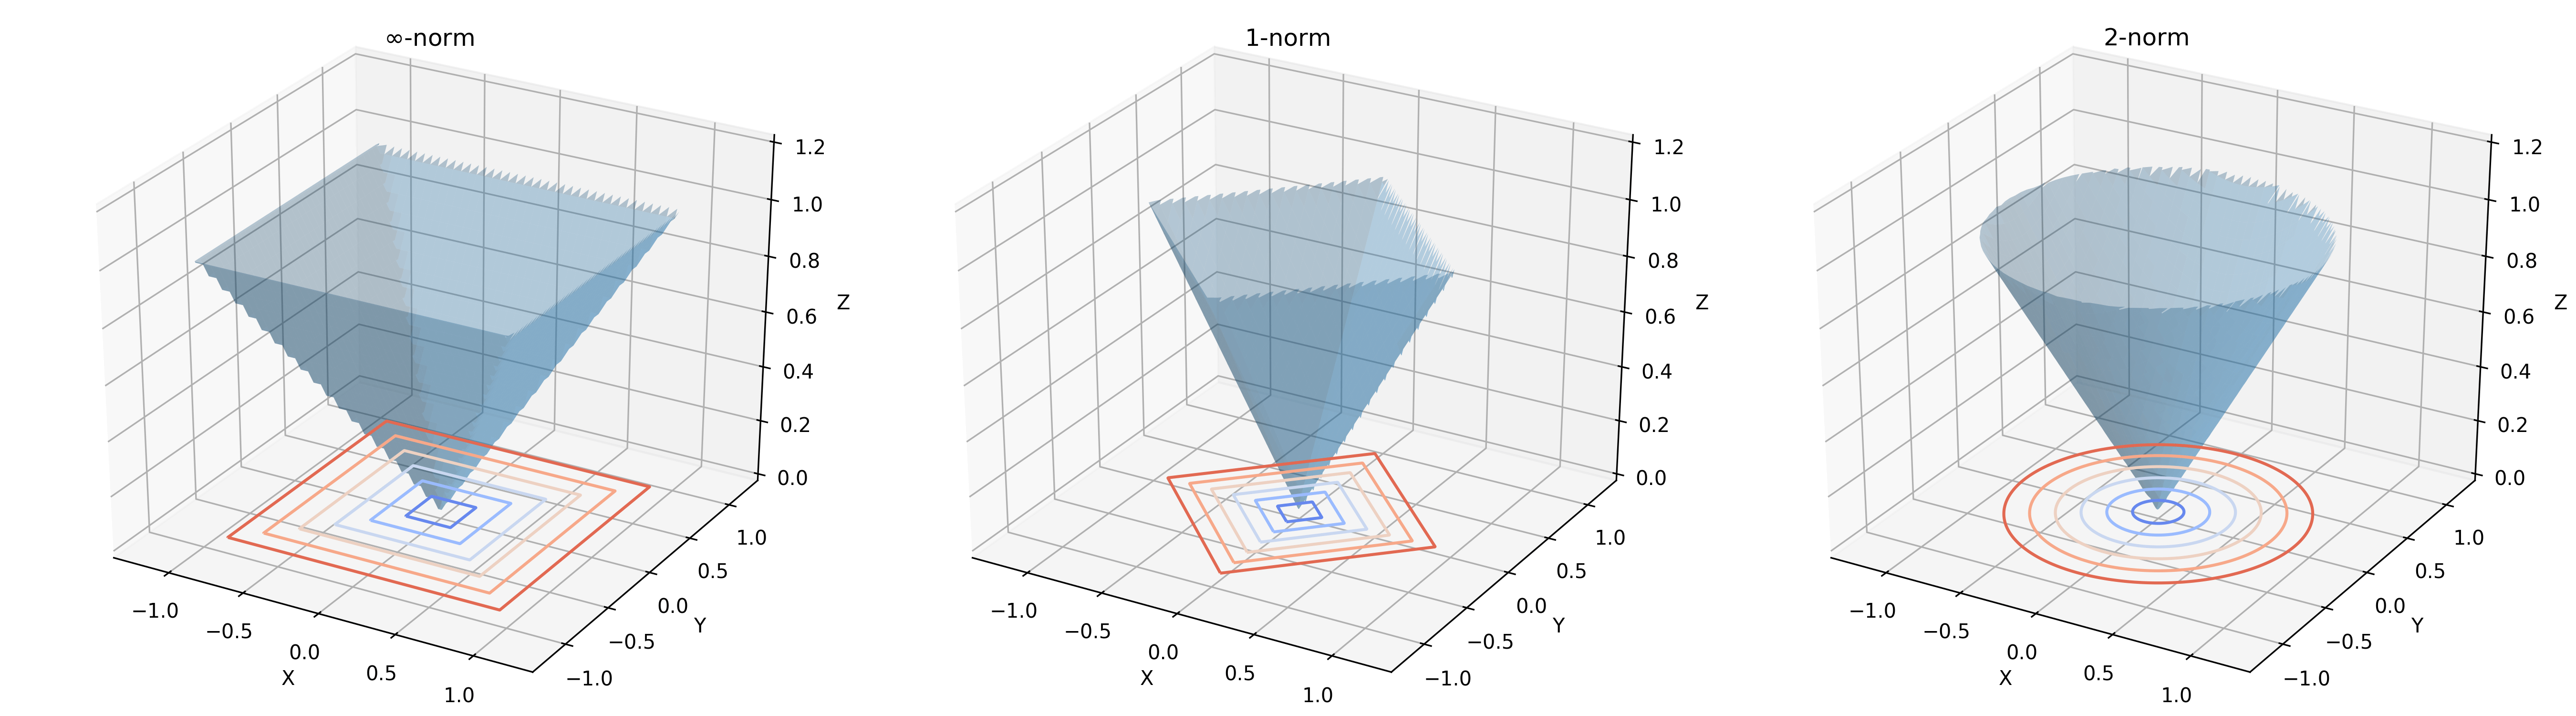
\includegraphics[width=.9\textwidth]{figures/1-1}
            \caption{Please refer to Appendix~\ref{S:appendix-1}}
        \end{figure}
    \item Given the vector norm $\norm{\cdot}_p$ for $\RR^n$, the induced norm for matrices $\mA\in\RR^{n\times n}$ is defined as
        \[
            \norm{\mA}_p = \max_{\vx\neq 0}\frac{\norm{\mA\vx}_p}{\norm{\vx}_p} = \max_{\norm{\vx}_p=1}\norm{\mA\vx}_p.
        \]
        Show that
        \begin{enumerate}[label=\roman*.]
            \item $\norm{\mA}_\infty=\max_{1\leq i\leq n}\sum_{j=1}^n\abs{a_{ij}}$;
                \begin{solution}{}{}
                    \begin{align*}
                        \norm{\mA}_\infty &= \max_{\norm{\vx}_\infty=1}\norm{\mA\vx}_\infty \\
                        &= \max_{\max_{1\leq j\leq n}\abs{x_j}=1}\max_{1\leq i\leq n}\sum_{j=1}^n\abs{a_{ij}x_j} \\
                        &\leq \max_{1\leq i\leq n}\sum_{j=1}^n\abs{a_{ij}} \\
                    \end{align*}
                    The equality holds when $x_j=\pm 1$ for $j=1,2,\ldots,n$.
                \end{solution}
            \item $\norm{\mA}_1=\max_{1\leq j\leq n}\sum_{i=1}^n\abs{a_{ij}}$;
                \begin{solution}{}{}
                    \begin{align*}
                        \norm{\mA}_1 &= \max_{\norm{\vx}_1=1}\norm{\mA\vx}_1 \\
                        &= \max_{\sum_{j=1}^n\abs{x_j}=1}\sum_{i=1}^n\sum_{j=1}^n\abs{a_{ij}x_j} \\
                        &\leq \max_{\sum_{j=1}^n\abs{x_j}=1}\sum_{j=1}^n\sum_{i=1}^n\abs{a_{ij}}\abs{x_j} = \max_{\sum_{j=1}^n\abs{x_j}=1}\sum_{j=1}^n\abs{x_j}\sum_{i=1}^n\abs{a_{ij}} \\
                        &\leq \max_{\sum_{j=1}^n\abs{x_j}=1}\sum_{j=1}^n\abs{x_j}\max_{1\leq j\leq n}\sum_{i=1}^n\abs{a_{ij}} = \max_{1\leq j\leq n}\sum_{i=1}^n\abs{a_{ij}}
                    \end{align*}
                    The equality holds when $j=\argmax_{1\leq j\leq n}\sum_{i=1}^n\abs{a_{ij}}$.
                \end{solution}
            \item $\norm{\mA}_2=\sqrt{\lambda_{\max}\qty(\mA^T\mA)}$.
                \begin{solution}{}{}
                    $\mA$ can be decomposed as $\vb{U}\vb*{\Sigma}\vb{V}^T$ by singular value decomposition, and the singular values on the diagonal are decreasing from top left to bottom right.
                    \begin{align*}
                        \norm{\mA}_2^2 &= \max_{\norm{\vx}_2=1} \norm{\mA\vx}_2^2 \\
                        &= \max_{\norm{\vx}_2=1} \qty(\mA\vx)^T\mA\vx = \max_{\norm{\vx}_2=1}\vx^T\vb{V}\vb*{\Sigma}^2\vb{V}^T\vx \\
                        &= \max_{\norm{\vx}_2=1}\vy^T\vb*{\Sigma}\vy = \max_{\norm{\vx}_2=1}\sum_{i=1}^n\sigma_iy_i^2 \\
                        &\leq \max_{\norm{\vx}_2=1}\max_{1\leq i\leq n}\sigma_i \vy^T\vy = \max_{\norm{\vx}_2=1}\max_{1\leq i\leq n}\sigma_i \vx^T\vx\\
                        &= \max_{1\leq i\leq n}\sigma_i = \lambda_{\max}\qty(\mA^T\mA).
                    \end{align*}
                    The equality holds when $\vx=\vb{V}\vb{e}_1$, where $\vb{e}_1=[1,0,\ldots,0]^T$.
                \end{solution}
        \end{enumerate}
\end{enumerate}



\section{Question 2}
\begin{enumerate}[label=(\alph*)]
    \item Use the method of undetermined coefficients to design third order accurate approximation to $u'(\bar{x})$ by using the discrete points $\bar{x}+h$, $\bar{x}$, $\bar{x}-h$, $\bar{x}-2h$.
        \begin{solution}{}{}
            According to Appendix~\ref{S:appendix-1}, we have
            \[
                u'(\bar{x}) = \frac{1}{h}\qty(\frac{u(\bar{x}-2h)}{6}-u(\bar{x}-h)+\frac{u(\bar{x})}{2}+\frac{u(\bar{x}+h)}{3}).
            \]
        \end{solution}
    \item Assuming $u(x)$ is smooth enough, compute the truncation error (leading term) for the finite difference formula above.
        \begin{solution}{}{}
            The leading term of the truncation error is of $\order{h^3}$, that is
            \[
                \frac{h^3}{12}u^{(4)}(\bar{x}).
            \]
        \end{solution}
    \item What is the truncation error if $u(x) = 4x^4 + 12x^3 + 6x^2 + x/2 + \pi$.
        \begin{solution}{}{}
            \begin{align*}
                u'(\bar{x}) &= \frac{1}{h}\qty(\frac{u(\bar{x}-2h)}{6}-u(\bar{x}-h)+\frac{u(\bar{x})}{2}+\frac{u(\bar{x}+h)}{3}) \\
                &= 16\bar{x}^3 + 36\bar{x}^2 + 12\bar{x} + \frac{1}{2}
            \end{align*}
            We have $u'(x)=16x^3 + 36x^2 + 12x + 1/2$, that is, the truncation error of this given function is $0$.
        \end{solution}
\end{enumerate}



\section{Question 3}
\begin{enumerate}[label=(\alph*)]
    \item For the following $N\times N$ matrix, show that all eigenvalues are given by $\lambda_p = a+2b\cos\tfrac{\pi p}{N+1}$ for $p=1,2,\ldots,N$.
        \[
            \qty[\begin{NiceArray}{CCCC}
                a & b      &        &   \\
                b & \Ddots & \Ddots &   \\
                  & \Ddots & \Ddots & b \\
                  &        & b      & a \\
            \end{NiceArray}]_{N\times N}
        \]
        \begin{solution}{}{}
            Please refer to Section~\ref{Q:4-1}.
        \end{solution}
\end{enumerate}



\section{Question 4}\label{Q:4-1}
\begin{enumerate}[label=(\alph*)]
    \item For the following $N\times N$ matrix, show that all eigenvalues are given by $\lambda_p = a+2\sqrt{bc}\cos\tfrac{\pi p}{N+1}$ for $p=1,2,\ldots,N$ and $bc>1$.
        \[
            \mA = \qty[\begin{NiceArray}{CCCC}
                a & c      &        &   \\
                b & \Ddots & \Ddots &   \\
                  & \Ddots & \Ddots & c \\
                  &        & b      & a \\
            \end{NiceArray}]_{N\times N}
        \]
        \begin{solution}{}{}
            The eigenvalues are $\lambda_p = a+2\sqrt{bc}\cos\tfrac{\pi p}{N+1}$, and the corresponding eigenvector $\vx^p$ has $j$th component
            \[
                \vx^p_j = \qty(\sqrt{\frac{b}{c}})^j \sin\qty(\frac{p\pi j}{N+1}).
            \]
            And $\vx^p_0=\vx^p_{N+1}=0$, if we want to show that $\mA\vx^p=\lambda_p\vx_p$, then we just need to show that $b\vx^p_{j-1}+a\vx^p_j+c\vx^p_{j+1}=\lambda_px^p_j$ for $j=1,2,\ldots,N$. We use the method of subtracting two sides to determine whether the two sides are equal by judging whether the result is zero. That is,
            \begin{align*}
                & b\vx^p_{j-1}+a\vx^p_j+c\vx^p_{j+1}-\lambda_px^p_j \\
                =& b\vx^p_{j-1}-2\sqrt{bc}\cos\frac{\pi p}{N+1}\vx^p_j+c\vx^p_{j+1} \\
                =& \qty(\frac{b}{c})^{(j-1)/2}\qty(b\sin\qty(\frac{\pi p(j-1)}{N+1})+b\sin\qty(\frac{\pi p(j+1)}{N+1})-2b\sin\qty(\frac{\pi pj}{N+1})\cos\qty(\frac{\pi p}{N+1})) \\
                =& \qty(\frac{b}{c})^{(j-1)/2}b\qty(\sin\qty(\frac{\pi p(j-1)}{N+1})+\sin\qty(\frac{\pi p(j+1)}{N+1})-2\sin\qty(\frac{\pi pj}{N+1})\cos\qty(\frac{\pi p}{N+1})) \\
                =& 0.
            \end{align*}
            The last step relies on $\sin(x+y)=\sin(x)\cos(y)+\cos(x)\sin(y)$. Since $N\times N$ matrix has at most $N$ eigenvalues, then $\lambda_p = a+2\sqrt{bc}\cos\tfrac{\pi p}{N+1}$ is all the eigenvalues the matrix has.
        \end{solution}
\end{enumerate}



\section{Question 5}
For the 2-point BVP with Neumann boundary conditions:
\[
    \begin{cases}
        u''(x) = f(x), & x\in(0, 1) \\
        u'(0) = u'(1) = 0 & \\
    \end{cases}
\]
\begin{enumerate}[label=(\alph*)]
    \item Set the grid points as $x_j=jh$ for $j=0,1,\ldots,N$ and $h=1/N$. Write down the central FD scheme for the main equation with using $u_j$ to approximate $u(x_j)$.
        \begin{solution}{}{}
            According to the central finite difference scheme, for $j=1,2,\ldots,N-1$ we have
            \[
                u''(x_j) = \frac{u(x_{j+1})-2u(x_j)+u(x_{j-1})}{h^2} = f(u_j)
            \]
            If we use $u'(\bar{x})=(u(\bar{x}+h)-u(\bar{x}))/h$ or $u'(\bar{x})=(u(\bar{x})-u(\bar{x})-h)/h$, we can approximate $u(x_0)$ by $u(x_1)$ and $u(x_N)$ by $u(x_{N-1})$. That is
            \[
                \frac{1}{h^2}
                \qty[\begin{NiceArray}{RRRRR}
                    -1 & 1      &        &        &    \\
                    1  & -2     & \Ddots &        &    \\
                       & \Ddots & \Ddots & \Ddots &    \\
                       &        & \Ddots & -2     & 1  \\
                       &        &        & 1      & -1 \\
                \end{NiceArray}]_{N-1\times N-1}
                \begin{bNiceMatrix}
                    u_1 \\ u_2 \\ \Vdots \\ \Vdots \\ u_{-1})
                \end{bNiceMatrix}
                =
                \begin{bNiceMatrix}
                    f(x_1) \\ f(x_2) \\ \Vdots \\ \Vdots \\ f(x_{N-1})
                \end{bNiceMatrix}.
            \]
        \end{solution}
    \item\label{tmp-1} Add two ``ghost'' points as $x_{-1}=-h$ and $x_{N+1}=1+h$, and two more variables $u_{-1}$ and $u_{N+1}$. Treat the boundary condition as $(u_1-u_{-1})/2h=0$, $(u_{N+1}-u_{N-1})/2h=0$. Assemble all the equations as $\mA\vb{U}=\vb{F}$ where $\vb{U}=[u_0, u_1, \ldots, u_N]^T$.
        \begin{solution}{}{}
            If we treat the boundary condition as the given way, we can approximate $u(x_{-1})$ by $u(x_1)$ and $u(x_{N+1})$ by $u(x_{N-1})$. Then all the equations can be assemble as $\mA\vb{U}=\vb{F}$ where $\vb{U}=[u_0,u_1,\ldots,u_N]^T$ and $\vb{F}=[f(x_0),f(x_1),\ldots,f(x_N)]^T$. Also, we have
            \[
                \mA = \frac{1}{h^2}
                \qty[\begin{NiceArray}{RRRRR}
                    -2 & 2      &        &        &    \\
                    1  & \Ddots & 1      &        &    \\
                       & \Ddots & \Ddots & \Ddots &    \\
                       &        & 1      & \Ddots & 1  \\
                       &        &        & 2      & -2 \\
                \end{NiceArray}]_{N+1\times N+1}
            \]
        \end{solution}
    \item Show that $\mA$ is singular, and find out when the system $\mA\vb{U}=\vb{F}$ has solutions.
        \begin{solution}{}{}
            We can first check the validity of the conclusion by MATLAB.
            \begin{matlabcode}{}
A = @(N) -2*eye(N+1) + diag([2, ones(1, N-1)], 1) + diag([ones(1, N-1), 2], -1);
for N = 1 : 99
    if det(A(N)) ~= 0
        disp(N);
    end
end
            \end{matlabcode}
            Then, we notice that the row sum of $\mA$ is 0, which means $\rank\mA\neq N$, this leads to the conclusion that $\mA$ is singular. As for when the system $\mA\vb{U}=\vb{F}$ has solutions, through the knowledge of linear algebra, we know that $\vb{F}$ must in the range space\footnote{In linear algebra, range space refers to the column space of a matrix, which is the set of all possible linear combinations of its column vectors.} of $\mA$.
        \end{solution}
    \item Find the kernel space of $\mA$.
        \begin{solution}{}{}
            The kernel space\footnote{The definition of kernel space is also appears in the computer field: System memory in Linux can be divided into two distinct regions: kernel space and user space. Kernel space is where the kernel (i.e., the core of the operating system) executes (i.e., runs) and provides its services.} is also called the null space, which is defined as
            \[
                \nullspace{\mA_{n\times n}} = \qty{\vx\in\RR^n \mid \mA\vx=\va{0}}.
            \]
            Therefor, the kernel space of $\mA$ is
            \[
                \spanof\qty{
                    \qty[\begin{NiceArray}{C}
                        1 \\ 1 \\ \Vdots \\ 1
                    \end{NiceArray}]_{N+1\times 1}
                }.
            \]
        \end{solution}
    \item Find out all eigenvalues and eigenvectors for the matrix $\mA$ given in \ref{tmp-1}.\todo[inline,color=green!40]{todo: re-derive it later.}
        \begin{solution}{}{}
            The non-zero eigenvalues of the matrix $\mA_{N+1\times N+1}$ is
            \[
                \lambda_p = -2 + 2\cos\frac{\pi p}{N},
            \]
            and the corresponding eigenvector $\vx^p$ has $j$th component
            \[
                \vx^p_j = \cos\qty(\frac{p\pi(j-1)}{N})
            \]
            for $p=0,1,\ldots,N$. We can then check the correctness of the result by MATLAB.
            \begin{matlabcode}{}
A = @(N) -2*eye(N+1) + diag([2, ones(1, N-1)], 1) + diag([ones(1, N-1), 2], -1);
lambda = @(N, p) -2 + 2*cos(pi*p/N);
x = @(N, p) cos(pi*p*(0:N)/N)';
error = @(N) N^2 * eps;
for N = 1 : 99
    for p = 0 : N
        delta = A(N)*x(N, p) - lambda(N, p)*x(N, p);
        if norm(delta, 1) > error(N)
            disp(['N=', num2str(N), '; p=', num2str(p), '; error=', num2str(norm(delta, 1))]);
        end
    end
end
            \end{matlabcode}
        \end{solution}
\end{enumerate}



\clearpage
\section{Appendix}\label{S:appendix-1}
\begin{appendices}
    \pythonfile{code/hw1.py}{\texttt{hw1.py}}
    \pythonfile{code/1_2.py}{\texttt{1\_2.py}}
    \pythonfile{code/1_2_sympy.py}{\texttt{1\_2\_sympy.py}}
\end{appendices}
